This appendix shows the electronic system designed to perform a complete characterization of the SiPM S13360-6075 model. This consists on three different PCBs\footnote{PCB, Printed Circuit Board}, shown in Figure \ref{fig:PCBs_LEDSpectrum}:

\begin{enumerate}
\item{} The first PCB, shown in Figure \ref{subfig:PCB1}, is used to organize the SiPMs and sensor temperature. This PCB place up to 8 different SiPMs and a temperature sensor and arrange their output signals on two HDMI connections. This PCB is placed inside a special black box, from Thorlabs company \cite{ThorlabsCompany}, that has a high degree of light tightness. This black box has a small hole of $1~\mm$ diameter, prepared to introduce an optical fiber\footnote{The optical fiber used is BCF-98 from Saint-Gobain company \cite{OpticalFibers}} to iluminate SiPMs with an incoherent light source. The light source utilized is a LED, model 430L from Thorlabs company \cite{LEDThorlabs}, which gives an spectrum shown in Figure \ref{subfig:LEDSpectrum}. The spectrum was experimentaly measured with a spectrometer and fitted to a Gaussian function. It can be seen that the emission peak of this LED is palced at $436.3$ with a FWHM\footnote{The FWHM parameter, Full Width at Half Maximum, of a Gaussian fit can be calculated from its sigma using the equation: FWHM$=2.35 \cdot{} \sigma$} of $19.1~\nano\meter$. With the help of this LED the light emission of the fibers used in TRITIUM experiment is simulated to calibrate the SiPMs at the working wavelength. 

\item{} The second PCB, shown in Figure \ref{subfig:PCB2}, sums the different signals of the SiPMs and amplify them by a factor $G=4187.5$ or $G=10761.88$, depending on the input resistance of the oscilloscope, $50~\varOmega$ or $1~\mega\varOmega$, respectively. This PCB uses a differential amplification that reduce the electronic noise of the system and is connected to the first PCB through two HDMI feedthroughs.

\item{} The third PCB, shown in Figure \ref{subfig:PCB3}, rearranges all the different input and output signals in an HDMI connection to avoid crosstalk between different signals. This PCB is connected to the second PCB trought a HDMI feedthrough.

The input signals are the supply voltage of the SiPMs and the supply voltage of the PCBs ($\pm 6~\volt$) and the output signals are the temperature sensor signal and the summed signal of all SiPMs. 

\end{enumerate}

\begin{figure}
\centering
    \begin{subfigure}[b]{0.5\textwidth}
    \centering
    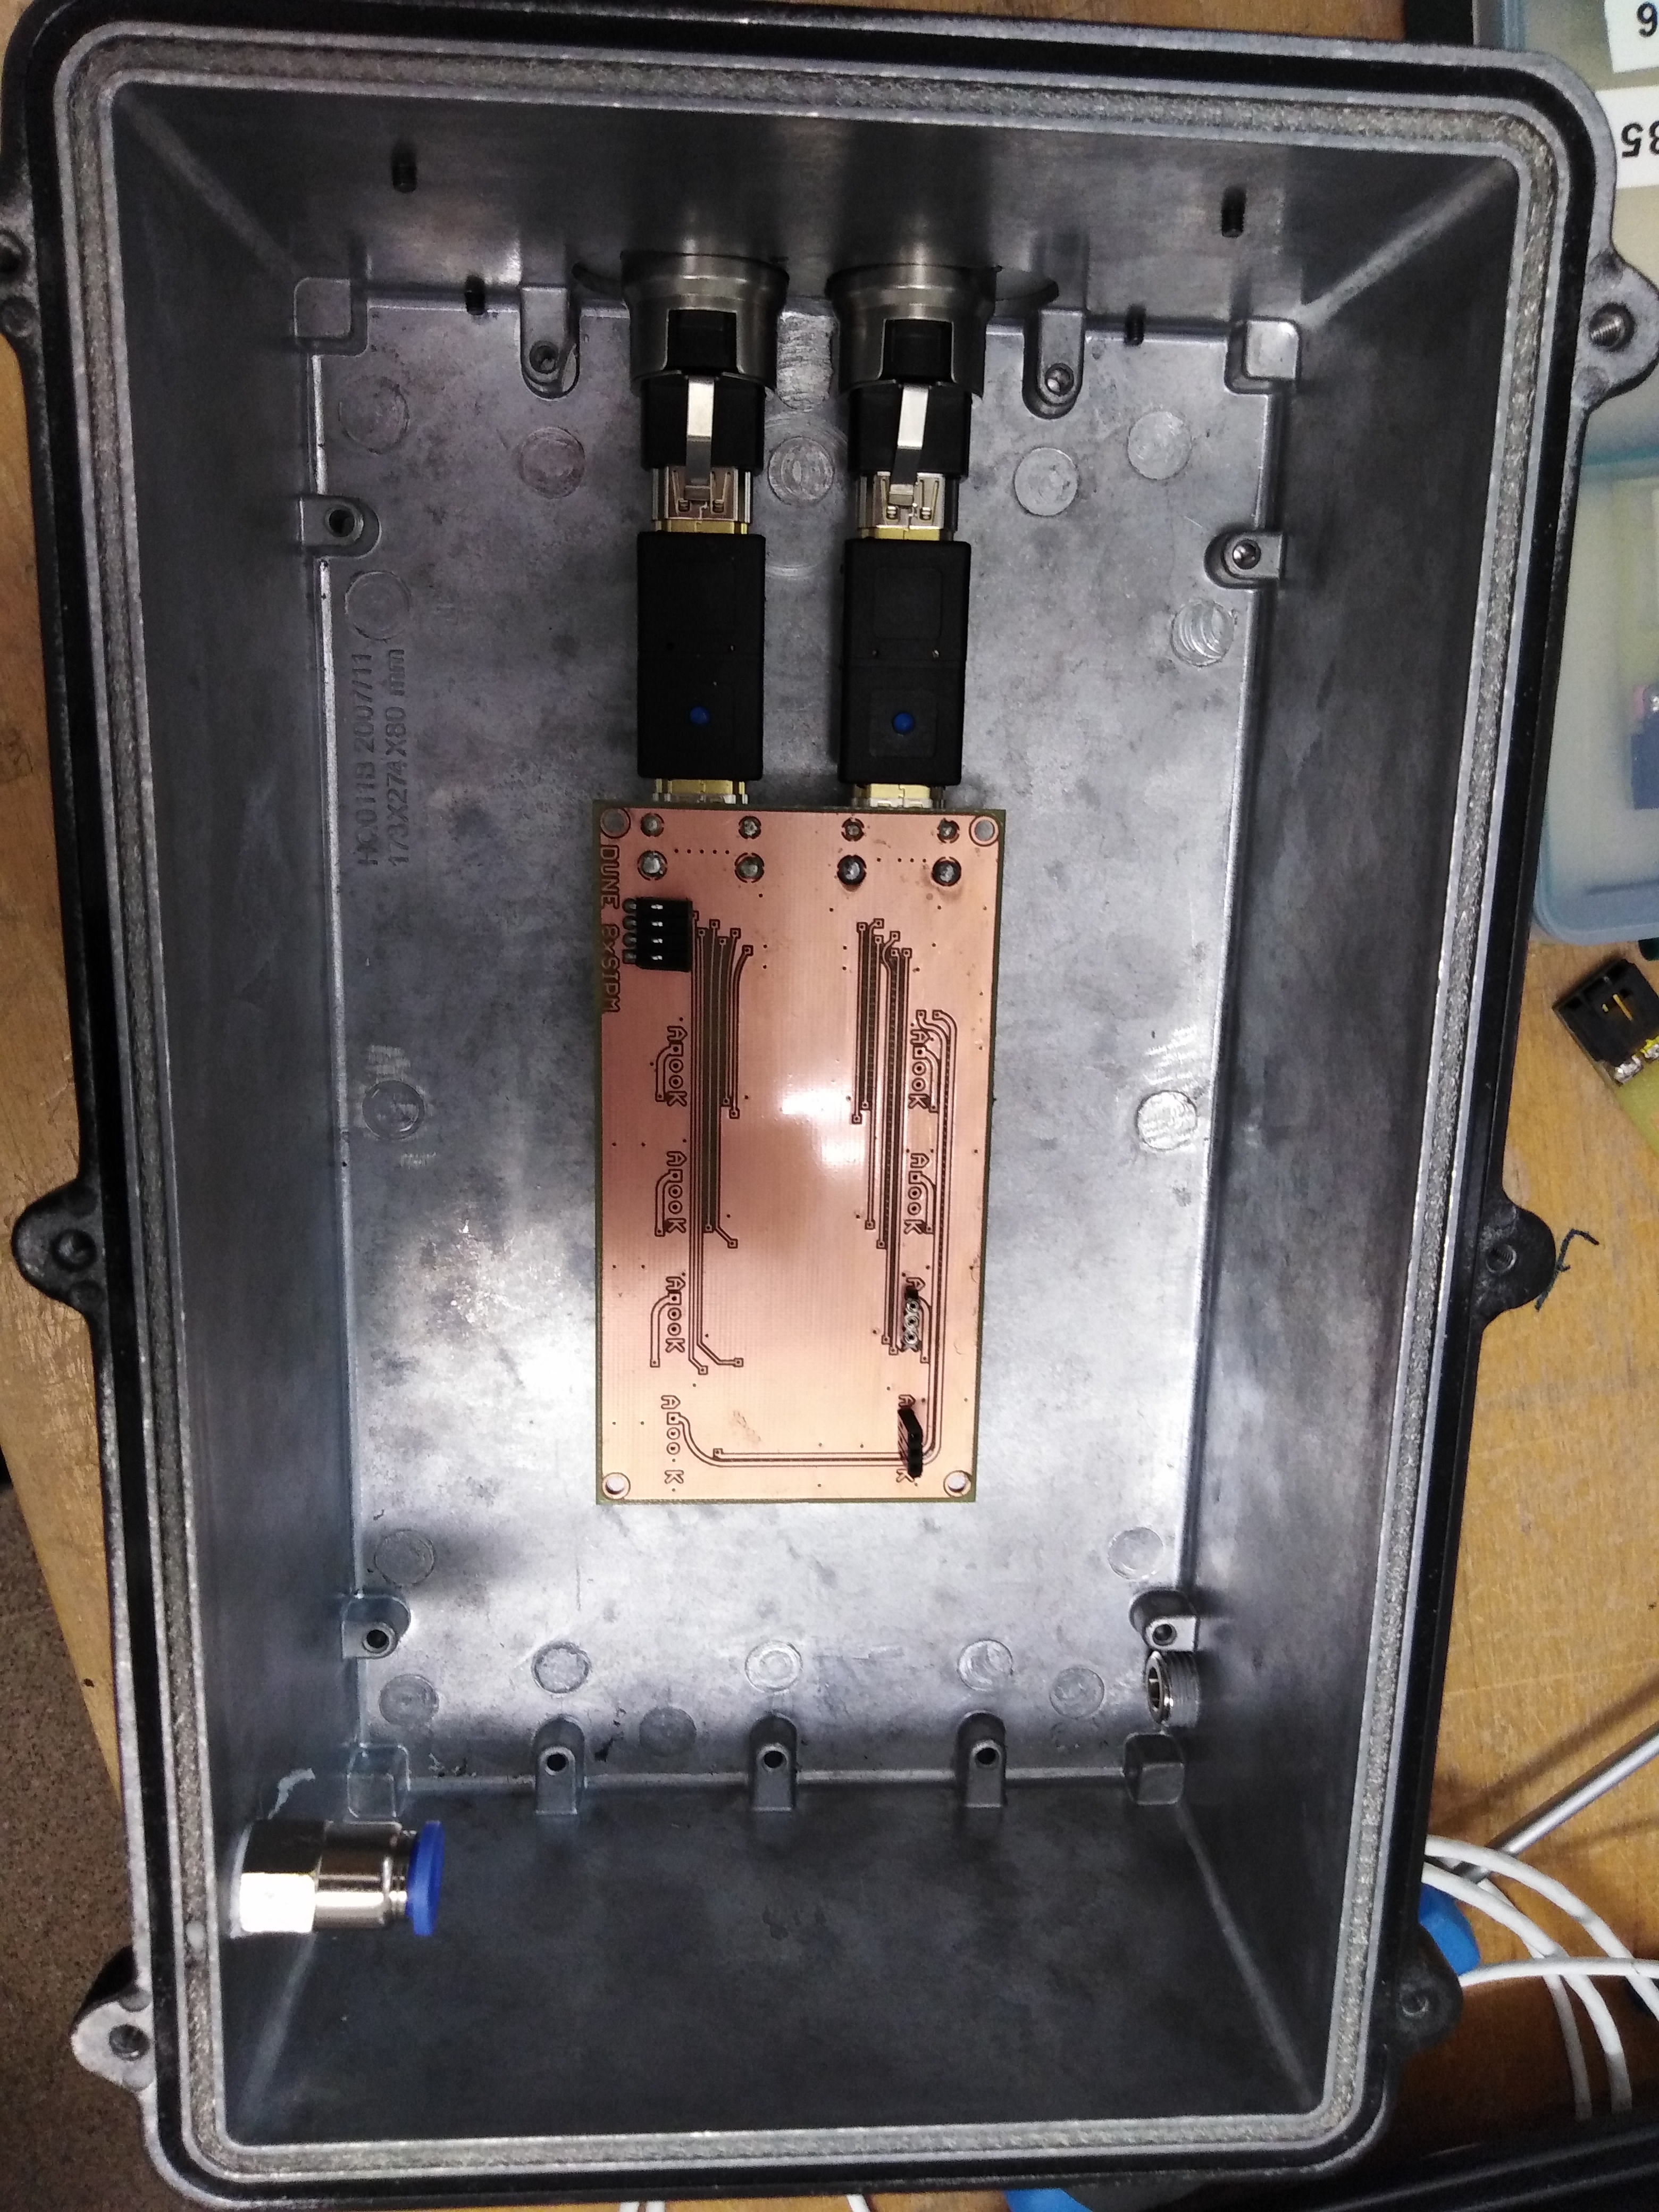
\includegraphics[width=\textwidth]{3DesignPrinciples/32Tritium_detector/PCB1_SiPM_Black_Box.jpg}  
    \caption{PCB 1 used to arrang 8 SiPMs and black box.\label{subfig:PCB1}}
    \end{subfigure}
    \hfill
    \begin{subfigure}[b]{0.45\textwidth}
    \centering
    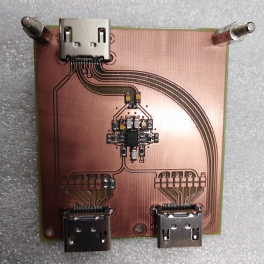
\includegraphics[width=\textwidth]{3DesignPrinciples/32Tritium_detector/PCB2_SIPMs.png}  
    \caption{PCB 2 used to sum and amplify the output signals of SiPMs.\label{subfig:PCB2}}
    \end{subfigure}
    \hfill
    \begin{subfigure}[b]{0.4\textwidth}
    \centering
    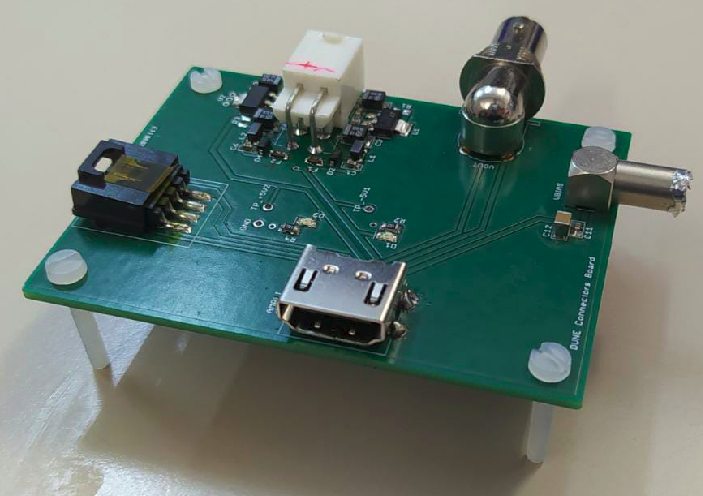
\includegraphics[width=\textwidth]{3DesignPrinciples/32Tritium_detector/PCB3_SiPMs.png}  
    \caption{PCB 3 used to rearrange the different singals of the system.\label{subfig:PCB3}}
    \end{subfigure}
    \hfill
    \begin{subfigure}[b]{0.5\textwidth}
    \centering
    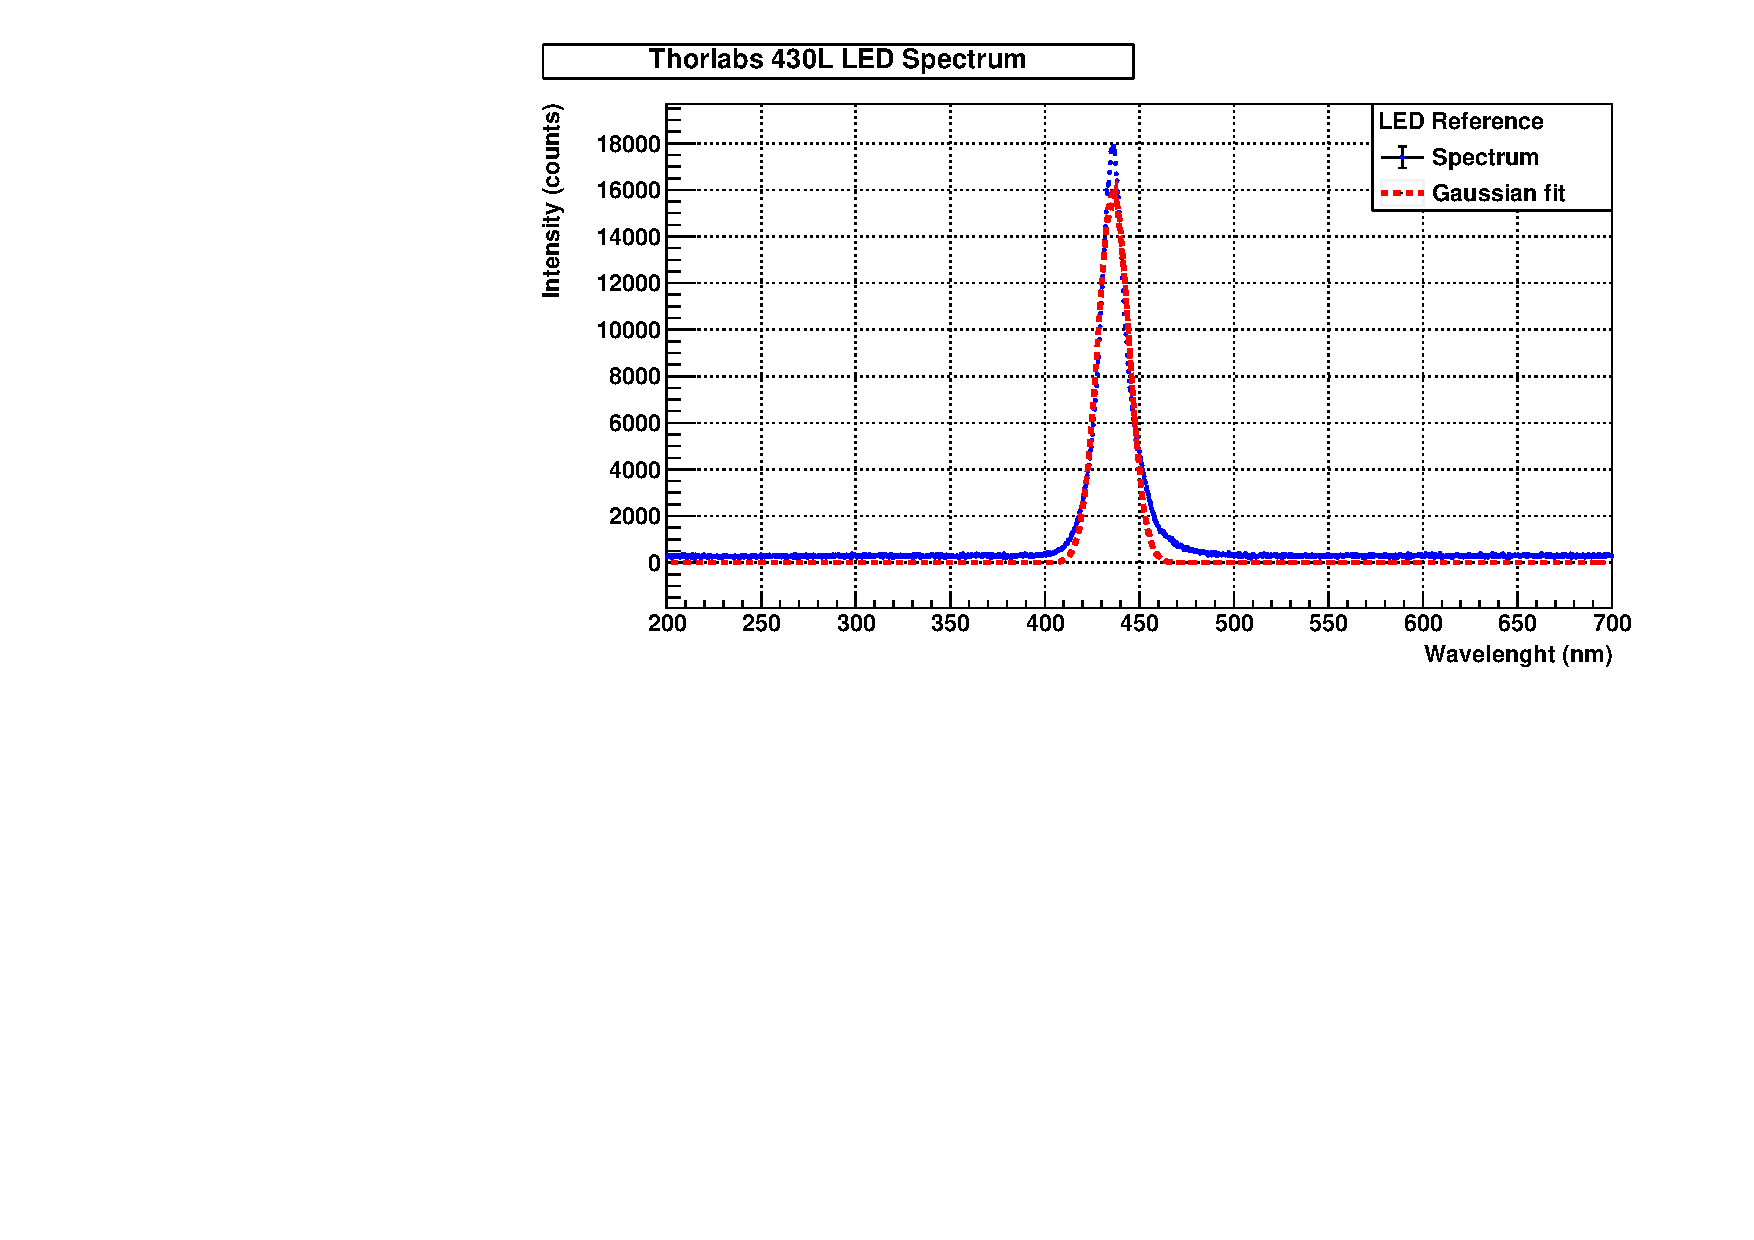
\includegraphics[width=\textwidth]{3DesignPrinciples/32Tritium_detector/LED_DUNE.pdf}  
    \caption{Emission spectrum of the LED.\label{subfig:LEDSpectrum}}
    \end{subfigure}
 \caption{Three PCBs used for the SiPM characterization and LED emission spectrum.}
 \label{fig:PCBs_LEDSpectrum}
\end{figure}

The output signal of the third PCB is connected to an oscilloscope, model MSO44X from Tektronix \cite{Oscilloscope}, that records the data which are subsequently analized by ROOT\footnote{ROOT is a framework for data processing, based on C ++ and object-oriented technology, developed at CERN and widely used in nuclear and particle physics.}.